% defer/rcufundamental.tex

\subsection{RCU Fundamentals}
\label{sec:defer:RCU Fundamentals}
\OriginallyPublished{Section}{sec:defer:RCU Fundamentals}{RCU Fundamentals}{Linux Weekly News}{PaulEMcKenney2007WhatIsRCUFundamentally}

RCU is made up of three fundamental mechanisms, the first being
used for insertion, the second being used for deletion, and the third
being used to allow readers to tolerate concurrent insertions and deletions.
Section~\ref{sec:defer:Publish-Subscribe Mechanism}
describes the publish-subscribe mechanism used for insertion,
Section~\ref{sec:defer:Wait For Pre-Existing RCU Readers}
describes how waiting for pre-existing RCU readers enabled deletion,
and
Section~\ref{sec:defer:Maintain Multiple Versions of Recently Updated Objects}
discusses how maintaining multiple versions of recently updated objects
permits concurrent insertions and deletions.
Finally,
Section~\ref{sec:defer:Summary of RCU Fundamentals}
summarizes RCU fundamentals.

\subsubsection{Publish-Subscribe Mechanism}
\label{sec:defer:Publish-Subscribe Mechanism}

RCU 읽기 쓰레드는 RCU 업데이트 쓰레드로부터 배제되지 않기 때문에, RCU 로
보호되는 데이터 구조는 읽기 쓰레드가 그걸 접근하는 사이에 변경될 수 있습니다.
이 접근된 데이터 아이템은 옮겨질 수도, 제거될 수도, 복제될 수도 있습니다.
이 데이터 구조는 읽기 쓰레드를 위해 ``잡혀져'' 있지 않기 때문에, 각 읽기
쓰레드의 액세스는 이 RCU 로 보호되는 데이터 아이템의 현재 버전에 대한 구독으로
생각될 수 있습니다.
그 부분들에 대해, 업데이트 쓰레드는 새로운 버전을 출시하는 것으로 생각될 수
있습니다.

Because RCU readers are not excluded by RCU updaters, an RCU-protected
data structure might change while a reader accesses it.
The accessed data item might be moved, removed, or replaced.
Because the data structure does not ``hold still'' for the reader,
each reader's access can be thought of as subscribing to the current
version of the RCU-protected data item.
For their part, updaters can be thought of as publishing new versions.

% @@@ Merge usage section into "Which to Choose?" and suggest choices.
% @@@ Should "RCU Exercises" move to "RCU Rescues"?

\begin{figure}[tb]
\centering
\resizebox{3in}{!}{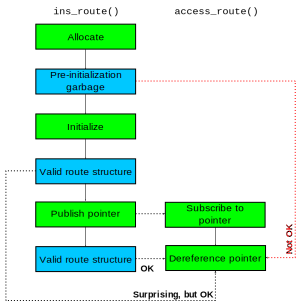
\includegraphics{defer/pubsub}}
\caption{Publication/Subscription Constraints}
\label{fig:defer:Publication/Subscription Constraints}
\end{figure}

불행히도,
Section~\ref{sec:toolsoftrade:Shared-Variable Shenanigans}
에서 다뤄지고
Section~\ref{sec:defer:Minimal Insertion and Deletion} 에서 한번 더 다뤄진
것처럼, 이 출시와 구독 작업에 평범한 액세스를 사용하는건 현명치 못한
처사입니다.
그대신 컴파일러와 CPU 모두에게 주의를 요할 것을 알려야 하는데, 이는
Figure~\ref{fig:defer:Publication/Subscription Constraints} 에서
Listing~\ref{lst:defer:Insertion and Deletion With Concurrent Readers}
의 \co{ins_route()} (와 그 호출자들) 그리고 \co{read_gptr()} 의 동시적 수행
사이의 상호작용을 그리며 보이고 있습니다.
\iffalse

Unfortunately, as laid out in
Section~\ref{sec:toolsoftrade:Shared-Variable Shenanigans}
and reiterated in
Section~\ref{sec:defer:Minimal Insertion and Deletion},
it is unwise to use plain accesses for these publication and subscription
operations.
It is instead necessary to inform both the compiler and the CPU
of the need for care, as can be seen from
Figure~\ref{fig:defer:Publication/Subscription Constraints},
which illustrates interactions between concurrent executions of
\co{ins_route()} (and its caller) and \co{read_gptr()} from
Listing~\ref{lst:defer:Insertion and Deletion With Concurrent Readers}.
\fi

Figure~\ref{fig:defer:Publication/Subscription Constraints}
에서의 \co{ins_route()} 열은 \co{ins_route()} 의 호출자가 새로운 \co{route}
구조체를 할당하는 걸 보이는데, 이는 초기화 전의 쓰레기값을 가지고 있을 겁니다.
이 호출자는 이어서 이 새로 할당된 구조체를 초기화 하고, 이어서 이 새로운
\co{route} 구조체로의 포인터를 출시하기 위해 \co{ins_route()} 를 호출합니다.
출시는 이 구조체의 내용물에 손대지 않으므로, 출시 후에도 그 내용물은
유효합니다.
\iffalse

The \co{ins_route()} column from
Figure~\ref{fig:defer:Publication/Subscription Constraints}
shows \co{ins_route()}'s caller allocating a new \co{route} structure,
which then contains pre-initialization garbage.
The caller then initializes the newly allocated structure, and then
invokes \co{ins_route()} to publish a pointer to the new \co{route}
structure.
Publication does not affect the contents of the structure, which
therefore remain valid after publication.
\fi

이 그림에서 \co{access_route()} 열은 구독되고 디레퍼런스 되는 포인터를
보입니다.
이 디레퍼런스 오퍼레이션은 초기화 전의 쓰레기값이 아닌 유효한 \co{route} 를
봐야만 하는데, 쓰레기 값을 레퍼런스 하는건 메모리 오염, 크래시, 그리고 행을
유발할 수 있기 때문입니다.
앞서 이야기 되었듯, 그런 쓰레기 값을 방지하는 것은 이 출시와 구독 오퍼레이션이
컴파일러와 CPU 모두에게 필요한 순서를 유지하도록 알려야 함을 의미합니다.
\iffalse

The \co{access_route()} column from this same figure shows
the pointer being subscribed to and dereferenced.
This dereference operation absolutely must see a valid \co{route}
structure rather than pre-initialization garbage because referencing
garbage could result in memory corruption, crashes, and hangs.
As noted earlier, avoiding such garbage means that the publish and
subscribe operations must inform both the compiler and the CPU of the
need to maintain the needed ordering.
\fi

출시는 \co{rcu_assign_pointer()} 을 통해 이루어지는데, 이 기능은
\co{ins_route()} 의 호출자의 초기화가 실제 출시 오퍼레이션의 포인터 저장 전으로
순서 이루어질 것을 보장합니다.
추가로, \co{rcu_assign_pointer()} 는 동시의 읽기 쓰레드가 해당 포인터의 이전 값
또는 새로운 값 중 하나만을 보지, 이 두 값이 합쳐진 이상한 값은 볼 수 없게끔
어토믹하게 이루어집니다.
이 요구사항은 C11 의 store-release 오퍼레이션으로 충족됩니다만, 실제 리눅스
커널 내에서 \co{rcu_assign_pointer()} 는 C11 store-release 와 대략적으로는
유사한 \co{smp_store_release()} 로 정의됩니다.
\iffalse

Publication is carried out by \co{rcu_assign_pointer()}, which ensures that
\co{ins_route()}'s callers initialization is ordered before the actual
publication operation's store of the pointer.
In addition, \co{rcu_assign_pointer()} must be atomic in the sense that 
concurrent readers see either the old value of the pointer or the new
value of the pointer, but not some mash-up of these two values.
These requirements are met by the C11 store-release operation,
and in fact in the Linux kernel, \co{rcu_assign_pointer()} is defined
in terms of \co{smp_store_release()}, which is roughly similar to
C11 store-release.
\fi

동시의 업데이트가 필요하다면, 같은 포인터로의 여러개의 동시적인
\co{rcu_assign_pointer()} 호출들 사이의 동기화 메커니즘이 필요할 것임을
알아두시기 바랍니다.
리눅스 커널 내에서는 락킹이 선택된 방법입니다만, 어떤 다른 동기화 메커니즘도
사용될 수 있습니다.
특히나 가벼운 동기화 메커니즘의 한 예는
Chapter~\ref{chp:Data Ownership} 의 데이터 소유권입니다: 각 포인터가 특정
쓰레드에 의해 소유되어 있다면, 해당 쓰레드는 해당 포인터로의
\co{rcu_assign_pointer()} 를 추가적인 동기화 오버헤드 없이 수행할 수 있을
겁니다.
\iffalse

Note that if concurrent updates are required, some sort of synchronization
mechanism will be required to mediate among multiple concurrent
\co{rcu_assign_pointer()} calls on the same pointer.
In the Linux kernel, locking is the mechanism of choice, but pretty
much any synchronization mechanism may be use.
An example of a particularly lightweight synchronization mechanism is
Chapter~\ref{chp:Data Ownership}'s data ownership: If each pointer is
owned by a particular thread, then that thread may execute
\co{rcu_assign_pointer()} on that pointer with no additional
synchronization overhead.
\fi

\QuickQuiz{}
	RCU 업데이트 쓰레드를 위한 데이터 소유권의 사용은 이 업데이트 작업이
	싱글쓰레드 버전의 코드와 동일한 인스트럭션들을 수행할 수 있다는 의미
	아닌가요?
	\iffalse

	Wouldn't use of data ownership for RCU updaters mean that
	the updates could use exactly the same sequence of instructions
	as would the corresponding single-threaded code?
	\fi
\QuickQuizAnswer{
	어떤 경우, 예를 들면 x86 이나 IBM mainframe 과 같이 store-release
	오퍼레이션이 하나의 스토어 인스트럭션을 만들어낼 뿐인 TSO
	시스템들에서는요.
	하지만, 완화된 순서 규칙의 시스템들에서는 메모리 배리어 또는
	store-release 인스트럭션 같은걸 추가적으로 수행해야만 합니다.
	또한, 데이터를 제거하는 것은 약간의 추가적인 작업을 필요로 하는데, 이
	제거된 데이터를 해제시키기 전에, 앞서 존재해온 읽기 쓰레드들을 기다려야
	하기 때문입니다.
	\iffalse

	Sometimes, for example, on TSO systems such as x86 or the IBM
	mainframe where a store-release operation emits a single store
	instruction.
	However, weakly ordered systems must also emit a memory barrier
	or perhaps a store-release instruction.
	In addition, removing data requires quite a bit of additional
	work because it is necessary to wait for pre-existing readers
	before freeing the removed data.
	\fi
} \QuickQuizEnd

구독은 \co{rcu_dereference()} 에 의해 수행되는데, 이 기능은 구독 오퍼레이션의
포인터 로드가 해당 포인터의 디레퍼런스 전에 이루어지도록 순서를 보장합니다.
\co{rcu_assign_pointer()} 와 유사하게, \co{rcu_dereference()} 는 로드되는 값이
하나의 스토어로 만들어진 값이어야 한다는 의미에서 어토믹해야 하는데, 예를 들어
컴파일러가 이 로드를 쪼개서 수행하면 안됩니다.\footnote{
	즉, 컴파일러는 이 로드를 여러개의 작은 로드들로 쪼개선 안됩니다,
	Section~\ref{sec:toolsoftrade:Shared-Variable Shenanigans} 의 ``load
	tearing'' 에서 설명된 것처럼요.}
불행히도, \co{rcu_dereference()} 를 위한 컴파일러 지원은 아직 완료되지
않았습니다~\cite{PaulEMcKennneyConsumeP0190R4,PaulEMcKenney2017markconsumeP0462R1,JFBastien2018P0750R1consume}.
그전까지는, 리눅스 커널은 volatile 로드, 각 CPU 아키텍쳐의 자세한 내용, 코딩
제약~\cite{PaulEMcKenney2014rcu-dereference}, 그리고 DEC Alpha~\cite{ALPHA2002}
위에서라면, 메모리 배리어 인스트럭션에 기대야 합니다.
하지만, 다른 아키텍쳐에서는 \co{rcu_dereference()} 는 보통 하나의 로드
인스트럭션을 만들어낼 뿐이어서 싱글쓰레드 버전 코드에서와 동일합니다.
\iffalse

Subscription is carried out by \co{rcu_dereference()}, which ensures that
the subscription operation's load from the pointer is ordered before the
dereference.
Similar to \co{rcu_assign_pointer()}, \co{rcu_dereference()} must be
atomic in the sense that the value loaded must be that from a single
store, for example, the compiler must not tear the load.\footnote{
	That is, the compiler must not break the load into multiple
	smaller loads, as described under ``load tearing'' in
	Section~\ref{sec:toolsoftrade:Shared-Variable Shenanigans}.}
Unfortunately, compiler support for \co{rcu_dereference()} is at best
a work in progress~\cite{PaulEMcKennneyConsumeP0190R4,PaulEMcKenney2017markconsumeP0462R1,JFBastien2018P0750R1consume}.
In the meantime, the Linux kernel relies on volatile loads, the details of
the various CPU architectures, coding
restrictions~\cite{PaulEMcKenney2014rcu-dereference},
and, on DEC Alpha~\cite{ALPHA2002}, a memory-barrier instruction.
However, on other architectures, \co{rcu_dereference()} typically
emits a single load instruction, just as would the equivalent single-threaded
code.
\fi
이 코딩 제약은
Section~\ref{sec:memorder:Address- and Data-Dependency Difficulties}
에서 더 자세히 설명되어 있습니다만, 평범한 필드 선택 (\qco{->} 도 잘
동작합니다.
읽기 쪽의 궁극적 성능을 필요로 하지 않는 소프트웨어라면 C11 acquire 로드를 대신
사용할 수 있을텐데, 이 기능은 우리가 필요한 순서규칙 외에도 몇가지 더 기능을
제공합니다, 비용이 조금 더 들긴 하지만요.
\co{rcu_dereference()} 를 위한 보다 가벼운 컴파일러 지원이 금방이든 나중이든
나오길 희망해 봅니다.
\iffalse
The coding restrictions are described in more detail in
Section~\ref{sec:memorder:Address- and Data-Dependency Difficulties},
however, the common case of field selection (\qco{->}) works quite well.
Software that does not require the ultimate in read-side performance
can instead use C11 acquire loads, which provide the needed ordering and
more, albeit at a cost.
It is hoped that lighter-weight compiler support for \co{rcu_dereference()}
will appear sooner rather than later.
\fi

요약해서, 포인터의 공개를 위한 \co{rcu_assign_pointer()} 사용과 그것들에 대한
구독을 위한 \co{rcu_dereference()} 의 사용은
Figure~\ref{fig:defer:Publication/Subscription Constraints} 에 그린 ``Not OK''
쓰레기값 로드 문제를 성공적으로 막습니다.
이 두 기능들은 따라서 새로운 데이터를 링크되어 있는 구조체에 동시의 읽기
쓰레드를 방해하지 않고 더할 수 있게 합니다.
\iffalse

In short, use of \co{rcu_assign_pointer()} for publishing pointers and
use of \co{rcu_dereference()} for subscribing to them successfully avoids the
``Not OK'' garbage loads depicted in
Figure~\ref{fig:defer:Publication/Subscription Constraints}.
These two primitives can therefore be used to add new data to linked
structures without disrupting concurrent readers.
\fi

\QuickQuiz{}
	하지만 읽기 쓰레드가 링크드 리스트를 순회하고 있는 사이에 업데이트
	쓰레드가 이 리스트에 여러 데이터 아이템을 넣고 빼고 있다고 생각해
	봅시다.
	구체적으로, 리스트가 처음엔 원소 A, B, 그리고 C 를 가지고 있었고 한
	업데이트 쓰레드가 원소 A 를 없애고 새로운 원소 D 를 이 리스트의
	마지막에 더했다고 생각해 봅시다.
	읽기 쓰레드는 \{A, B, C, D\} 를 볼수도 있는데, 이 원소들이 존재하는
	조합은 결코 실제로 존재한 적 없는 것입니다!
	대체 어떤 대안적인 세계에서는 이걸 가지고 ``동시의 읽기 쓰레드를
	방해하지 않는다''고 할 수 있는 거죠???
	\iffalse

	But suppose that updaters are adding and removing multiple data
	items from a linked list while a reader is iterating over that
	same list.
	Specifically, suppose that a list initially contains elements
	A, B, and C, and that an updater removes element A and then
	adds a new element D at the end of the list.
	The reader might well see \{A, B, C, D\}, when that sequence of
	elements never actually ever existed!
	In what alternate universe would that qualify as ``not disrupting
	concurrent readers''???
	\fi
\QuickQuizAnswer{
	순회하는 읽기 쓰레드가 이 순회 기간 전체에 있어 존재한 원소들을
	순회하기만 하면 된다는 세계에서입니다.
	이 예에서, 이는 원소 B 와 C 가 될 겁니다.
	원소 A 와 D 는 이 순회의 한 부분에서만 존재했기 때문에, 읽기 쓰레드는
	그것들을 순회할 수 있지만, 그게 강요되진 않습니다.

	이보다 강한 일관성이 필요하다면, 더 높은 비용의 동기화 메커니즘이
	필요한데, 예를 들면 시퀀스 락킹이나 reader-writer 락킹입니다.
	하지만 더 강한 일관성이 필요하지 \emph{않다면} (많은 경우에
	그렇습니다), 왜 더 높은 비용을 내겠어요?
	\iffalse

	In the universe where an iterating reader is only required to
	traverse elements that were present throughout the full duration
	of the iteration.
	In the example, that would be elements B and C.
	Because elements A and D were each present for only part of the
	iteration, the reader is permitted to iterate over them, but not
	obliged to.

	If stronger consistency is required, then higher-cost
	synchronization mechanisms are required, for example, sequence
	locking or reader-writer locking.
	But if stronger consistency is \emph{not} required (and it very often
	is not), then why pay the higher cost?
	\fi
} \QuickQuizEnd

링크된 구조체에 읽기 쓰레드를 방해하지 않고 데이터를 넣는 건 좋은 일인데, 이는
읽기 쪽 비용을 싱글쓰레드 버전 읽기 쓰레드에 비해 비용을 높이지 않기 때문에
그렇습니다.
하지만, 대부분의 경우엔 데이터를 지우는 것도 필요하고, 이는 다음 섹션에서
다룹니다.
\iffalse

Adding data to a linked structure without disrupting readers is a good thing,
as are the cases where this can be done with no added read-side cost compared
to single-threaded readers.
However, in most cases it is also necessary to remove data, and this is the
subject of the next section.
\fi

\subsubsection{Wait For Pre-Existing RCU Readers}
\label{sec:defer:Wait For Pre-Existing RCU Readers}

가장 기본적인 형태에서, RCU 는 일들이 끝나기를 기다리는 방법입니다.
물론, RCU 외에도 일들이 끝나길 기다리는 훌륭한 방법들이 여럿 있는데, 레퍼런스
카운팅, reader-writer lock, 이벤트 등등이 포함됩니다.
RCU 의 커다란 장점은 (대략) 20,000 개의 서로 다른 일들을 명시적으로 그 모든
것들을 각각 정보를 쫓아가지 않으면서 성능 하락, 확장성 제한, 복잡한 데드락
시나리오, 그리고 명시적으로 정보를 쫓는 방법에서는 필연적인 메모리 누수 문제를
걱정할 필요 없이 기다릴 수 있다는 겁니다.
\iffalse

In its most basic form, RCU is a way of waiting for things to finish.
Of course, there are a great many other ways of waiting for things to
finish, including reference counts, reader-writer locks, events, and so on.
The great advantage of RCU is that it can wait for each of
(say) 20,000 different things without having to explicitly
track each and every one of them, and without having to worry about
the performance degradation, scalability limitations, complex deadlock
scenarios, and memory-leak hazards that are inherent in schemes
using explicit tracking.
\fi

RCU 의 경우에, 기다려지고 있는 일들은 \emph{RCU read-side 크리티컬 섹션} 이라
불립니다.
Section~\ref{sec:defer:Toy Implementation}
에서 힌트를 준 것처럼, RCU read-side 크리티컬 섹션은 \co{rcu_read_lock()}
함수로 시작되고, 그에 연관되는 \co{rcu_read_unlock()} 함수로 종료됩니다.
RCU read-side 크리티컬 섹션들은 중첩될 수 있고, 어떤 코드든 그 코드가
quiescent state 를 갖지 않는 한 그 안에 들어갈 수 있는데, 예를 들어 리눅스
커널에서는 컨텍스트 스위치가 quiescent state 중 하나이기 때문에 RCU read-side
크리티컬 섹션 내에서 sleep 을 하는건 불법입니다.\footnote{
	하지만, SRCU~\cite{PaulEMcKenney2006c} 라고 하는 특수한 형태의 RCU 는
	SRCU read-side 크리티컬 섹션 내에서의 sleep 을 허용합니다.}
여러분이 이 규약을 준수한다면, 여러분은 \emph{모든} 이전부터 존재한 RCU
read-side 크리티컬 섹션이 완료되길 기다리는데 RCU 를 사용할 수 있으며,
\co{synchronize_rcu()} 는 이 실제 기다림을 하는 간접적 수단을
사용합니다~\cite{MathieuDesnoyers2012URCU,McKenney:2013:SDS:2483852.2483867}.
\iffalse

In RCU's case, each of the things waited on is called an
\emph{RCU read-side critical section}.
As hinted at in
Section~\ref{sec:defer:Toy Implementation}, an RCU read-side critical
section starts with an \co{rcu_read_lock()} primitive, and ends with a
corresponding \co{rcu_read_unlock()} primitive.
RCU read-side critical sections can be nested, and may contain pretty
much any code, as long as that code does not contain a quiescent state,
for example, within the Linux kernel, it is illegal to sleep within
an RCU read-side critical section because a context switch is a quiescent
state.\footnote{
	However, a special form of RCU called SRCU~\cite{PaulEMcKenney2006c}
	does permit general sleeping in SRCU read-side critical sections.}
If you abide by these conventions, you can use RCU to wait for \emph{any}
pre-existing RCU read-side critical section to complete, and
\co{synchronize_rcu()} uses indirect means to do the actual
waiting~\cite{MathieuDesnoyers2012URCU,McKenney:2013:SDS:2483852.2483867}.
\fi

\begin{figure}[tb]
\centering
\resizebox{3in}{!}{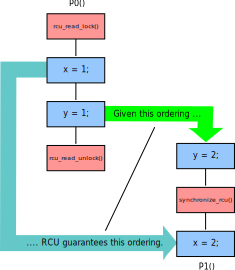
\includegraphics{defer/RCUGuaranteeFwd}}
\caption{RCU Reader and Later Grace Period}
\label{fig:defer:RCU Reader and Later Grace Period}
\end{figure}

RCU read-side 크리티컬 섹션과 뒤의 RCU grace period 사이의 관계는
Figure~\ref{fig:defer:RCU Reader and Later Grace Period} 에 그린 것처럼 if-then
관계입니다.
특정 크리티컬 섹션의 어떤 부분이 특정 grace period 의 시작을 앞선다면, RCU 는
이 크리티컬 섹션 전체가 이 grace period 의 종료를 앞서게 될 것을 보장합니다.
이 그림에서, \co{P0()} 의 \co{y} 접근이 \co{P1()} 의 해당 변수로의 접근을
앞서므로, \co{P0()} 의 \co{x} 로의 접근은 \co{P1()} 의 액세스를 앞설 겁니다.
이 경우, \co{y} 의 마지막 값이 2라면, \co{x} 의 마지막 값 역시 2가 될 것이
보장됩니다.
\iffalse

The relationship between an RCU read-side critical section and a later
RCU grace period is an if-then relationship, as illustrated by
Figure~\ref{fig:defer:RCU Reader and Later Grace Period}.
If any portion of a given critical section precedes the beginning of
a given grace period, then RCU guarantees that all of that critical
section will precede the end of that grace period.
In the figure, because \co{P0()}'s access to \co{y} precedes
\co{P1()}'s access to this same variable, it is guaranteed that
\co{P0()}'s access to \co{x} will precede \co{P1()}'s access.
In this case, if \co{y}'s final value is 2, then \co{x}'s
final value is guaranteed to also be 2.
\fi

\QuickQuiz{}
	Figure~\ref{fig:defer:RCU Reader and Later Grace Period}
	에서 \co{x} 와 \co{y} 의 마지막 값은 다른 어떤 값이 될수도 있을까요?
	\iffalse

	What other final values of \co{x} and \co{y} are possible in
	Figure~\ref{fig:defer:RCU Reader and Later Grace Period}?
	\fi
\QuickQuizAnswer{
	\co{x == 2 && y == 2} 일 가능성은 앞의 글에서 설명되었습니다.
	\co{y == 2} 가 \co{x == 2} 일 것을 의미하므로, \co{x == 1 && y == 2} 는
	불가능함을 알고 있습니다.
	뒤의 토의는 \co{x == 1 && y == 1} 과 \co{x == 2 && y == 1} 이 가능함을
	보입니다.
	\iffalse

	The \co{x == 2 && y == 2} possibility was called out in the text.
	Given that \co{y == 2} implies \co{x == 2}, we know that
	\co{x == 1 && y == 2} is forbidden.
	The following discussion will show that both
	\co{x == 1 && y == 1} and \co{x == 2 && y == 1} are possible.
	\fi
} \QuickQuizEnd

\begin{figure}[tb]
\centering
\resizebox{3in}{!}{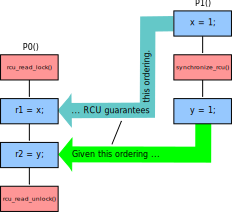
\includegraphics{defer/RCUGuaranteeRev}}
\caption{RCU Reader and Earlier Grace Period}
\label{fig:defer:RCU Reader and Earlier Grace Period}
\end{figure}

RCU read-side 크리티컬 섹션과 그 전의 RCU grace period 사이의 관계 역시 if-then
관계이며,
Figure~\ref{fig:defer:RCU Reader and Earlier Grace Period} 에 그려져 있습니다.
특정 크리티컬 섹션의 어떤 부분이 특정 grace period 의 종료를 뒤따른다면, RCU 는
이 크리티컬 섹션의 모든 부분이 이 grace period 의 시작을 뒤따를 것을
보장합니다.
이 그림에서, \co{P0()} 의 \co{x} 로의 접근이 \co{P1()} 의 같은 변수로의 접근을
뒤따르므로, \co{P0()} 의 \co{y} 로의 접근은 \co{P1()} 의 접근을 앞설 것이
보장됩니다.
이 경우, 만약 \co{x} 의 마지막 값이 1이라면, \co{y} 의 마지막 값 역시 1일 것이
보장됩니다.
\iffalse

The relationship between an RCU read-side critical section and an earlier
RCU grace period is also an if-then relationship, as illustrated by
Figure~\ref{fig:defer:RCU Reader and Earlier Grace Period}.
If any portion of a given critical section follows the end of
a given grace period, then RCU guarantees that all of that critical
section will follow the beginning of that grace period.
In the figure, because \co{P0()}'s access to \co{x} follows
\co{P1()}'s access to this same variable, it is guaranteed that
\co{P0()}'s access to \co{y} will precede \co{P1()}'s access.
In this case, if \co{x}'s final value is 1, then \co{y}'s
final value is guaranteed to also be 1.
\fi

\begin{figure}[tb]
\centering
\resizebox{3in}{!}{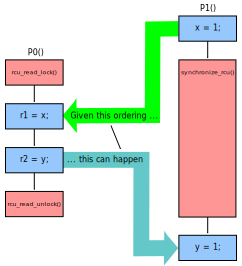
\includegraphics{defer/RCUGuaranteeMid}}
\caption{RCU Reader Within Grace Period}
\label{fig:defer:RCU Reader Within Grace Period}
\end{figure}

마지막으로,
Figure~\ref{fig:defer:RCU Reader Within Grace Period} 에 보인 것처럼, RCU
read-side 크리티컬 섹션은 RCU grace period 에 의해 완전히 중복될 수 있습니다.
여기서 \co{x} 의 마지막 값은 1이고 \co{y} 의 마지막 값은 2 입니다.
\iffalse

Finally, as shown in
Figure~\ref{fig:defer:RCU Reader Within Grace Period},
an RCU read-side critical section can be completely overlapped by
an RCU grace period.
In this case, \co{x}'s final value is 1 and \co{y}'s final value is 2.
\fi

하지만, \co{x} 의 마지막 값이 2 이고 \co{y} 의 마지막 값이 1일 수는 없습니다.
이는 RCU read-side 크리티컬 섹션은 하나의 grace period 내에 완전히 파묻혀서,
감춰져 버릴 수 있음을 의미합니다.
RCU 의 wait-for-readers 보장은 따라서 두개의 부분으로 이루어집니다:
(1)~만약 특정 RCU read-side 크리티컬 섹션의 어느 부분이 특정 grace period 의
시작을 앞선다면, 이 크리티컬 섹션의 모든 부분이 이 grace period 의 끝을 앞선다.
(2)~만약 특정 RCU read-side 크리티컬 섹션의 어느 부분이 특정 grace period 의
끝을 뒤따른다면, 이 크리티컬 섹션의 모든 부분이 이 grace period 의 시작을
뒤따른다.
이 정의는 거의 모든 RCU 기반 알고리즘에 충분합니다만, 더 많은 걸 원하는
사람들을 위해, RCU 의 간단한 수행에 대한 정형적 모델이 리눅스 커널 v4.17 과 그
뒤 버전들의 부분으로 사용 가능하며,
Section~\ref{sec:formal:Axiomatic Approaches and RCU} 에 설명되어 있습니다.
추가로, RCU 의 순서 특성은 Section~\ref{sec:memorder:RCU} 에 훨씬 자세히
설명되어 있습니다.
\iffalse

However, it cannot be the case that \co{x}'s final value is 2 and \co{y}'s
final value is 1.
This would mean that an RCU read-side critical section had completely
overlapped a grace period, which is forbidden.
RCU's wait-for-readers guarantee therefore has two parts:
(1)~If any part of a given RCU read-side critical section precedes
the beginning of a given grace period, then the entirety of that
critical section precedes the end of that grace period.
(2)~If any part of a given RCU read-side critical section follows
the end of a given grace period, then the entirety of that
critical section follows the beginning of that grace period.
This definition is sufficient for almost all RCU-based algorithms, but
for those wanting more,
simple executable formal models of RCU are available
as part of Linux kernel v4.17 and later, as discussed in
Section~\ref{sec:formal:Axiomatic Approaches and RCU}.
In addition, RCU's ordering properties are examined in much
greater detail in Section~\ref{sec:memorder:RCU}.
\fi

RCU 의 wait-for-readers 기능이
Figure~\ref{fig:defer:RCU Reader and Later Grace Period}-\ref{fig:defer:RCU Reader Within Grace Period}
에서 보인 것처럼 변수로의 값 할당 순서를 위해 가끔은 사용되지만,
Section~\ref{sec:defer:Introduction to RCU} 에서 한것처럼 연결된 구조체에서
제거된 데이터 원소를 안전히 해제하는데에 더 자주 사용됩니다.
일반화된 프로세스는 다음 pseudocode 로 설명됩니다:
\iffalse

Although RCU's wait-for-readers capability really is sometimes used to
order the assignment of values to variables as shown in
Figures~\ref{fig:defer:RCU Reader and Later Grace Period}-\ref{fig:defer:RCU Reader Within Grace Period},
it is more frequently used to safely free data elements removed from
a linked structure, as was done in
Section~\ref{sec:defer:Introduction to RCU}.
The general process is illustrated by the following pseudocode:
\fi

\begin{enumerate}
\item	변경을 만드는데, 예를 들어 링크드 리스트에서 원소를 제거합니다.
\item	모든 이전부터 존재한 RCU read-side 크리티컬 섹션이 완전히 종료되길
	기다립니다 (예를 들면, \co{synchronize_rcu()} 를 사용해서).
\item	해제를 진행합니다, 예를 들어 앞서 교체된 원소를 메모리에서
	해제시킵니다.
\iffalse

\item	Make a change, for example, remove an element from a linked list.
\item	Wait for all pre-existing RCU read-side critical sections to
	completely finish (for example, by using
	\co{synchronize_rcu()}).
\item	Clean up, for example, free the element that was replaced above.
\fi
\end{enumerate}

\begin{figure}[tb]
\centering
\resizebox{3in}{!}{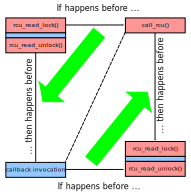
\includegraphics{defer/RCUGPordering}}
\caption{RCU Grace-Period Ordering Guarantees}
\label{fig:defer:RCU Grace-Period Ordering Guarantees}
\end{figure}

이 보다 추상적인 프로시져는 특정 리트머스 테스트에 구체적인
Figures~\ref{fig:defer:RCU Reader and Later Grace Period}--\ref{fig:defer:RCU Reader Within Grace Period}
보다 더 추상적인 다이어그램을 필요로 합니다.
Figure~\ref{fig:defer:RCU Grace-Period Ordering Guarantees}
가 이 필요를 충족하는데, 좌상단과 우하단의 RCU read-side 크리티컬 섹션이
우상단의 \co{call_rcu()} 로 시작되고 좌하단의 연관된 콜백 호출로 끝나는 grace
period 와 어떻게 순서지어지는지 보이고 있습니다.
이 다이어그램은 RCU 의 wait-for-readers 기능을 보이고 있습니다:
주어진 grace period 에 대해, 각 읽기 쓰레드는 이 grace period 의 끝 전에
끝나거나 이 grace period 의 시작 후에 시작합니다.
\iffalse

This more abstract procedure requires a more abstract diagram than
Figures~\ref{fig:defer:RCU Reader and Later Grace Period}--\ref{fig:defer:RCU Reader Within Grace Period},
which are specific to a particular litmus test.
Figure~\ref{fig:defer:RCU Grace-Period Ordering Guarantees}
fills this need, showing how the RCU read-side critical sections
in the upper left and lower right are ordered with a grace period
that starts with a \co{call_rcu()} at the upper right and ends
with the invocation of the corresponding callback at the lower left.
This diagram illustrates RCU's wait-for-readers functionality:
Given a grace period, each reader either ends before the end of that
grace period or starts after the beginning of that grace period.
\fi

RCU 읽기 쓰레드가 업데이트가 진행 중일 때에도 진행을 낼 수 있다는 걸 놓고 보면,
다른 읽기 쓰레드는 데이터 구조의 상태에 동의하지 않을 수도 있는데, 다음
섹션에서 이 주제를 다룹니다.
\iffalse

Given that RCU readers can make forward progress while updates
are in progress, different readers might disagree about the state
of the data structure, a topic taken up by the next section.
\fi

\subsubsection{Maintain Multiple Versions of Recently Updated Objects}
\label{sec:defer:Maintain Multiple Versions of Recently Updated Objects}

이 섹션은 RCU 가 데이터의 여러 버전을 유지함으로써 동기화에 자유로운 읽기
쓰레드를 어떻게 가능하게 하는지 논합니다.
이 토론은
Section~\ref{sec:defer:Minimal Insertion and Deletion} 의
Figure~\ref{fig:defer:Deletion With Concurrent Readers}
에서의 여러 버전들에 대한 소개 위에서 이루어지는데, 즉, 동시에 \co{del_route()}
(Listing~\ref{lst:defer:Insertion and Deletion With Concurrent Readers} 을
참고하세요) 와 동시에 수행중인 읽기 쓰레드는 과거의 \co{route} 구조체나 텅빈
리스트를 볼 수도 있습니다만, 어쨌든 올바른 결과만을 얻습니다.
물론, Figure~\ref{fig:defer:Insertion With Concurrent Readers} 을 자세히 들여다
보면 알 수 있듯이 \co{ins_route()} 호출 역시 동시의 읽기 쓰레드들이 다른
버전들을 보게 만들 수 있습니다: 최초의 텅빈 리스트 또는 새로 삽입된 \co{route}
구조체.
레퍼런스 카운팅
(Section~\ref{sec:defer:Reference Counting})
과 해저드 포인터
(Section~\ref{sec:defer:Hazard Pointers})
역시 동시의 읽기 쓰레드가 다른 값을 보게 할 수 있지만, RCU 의 극단적으로 가벼운
읽기 쓰레드는 읽기 쓰레드가 그럴 가능성을 높입니다.
\iffalse

This section discusses how RCU accommodates synchronization-free readers
by maintaining multiple versions of data.
This discussion builds on the introduction of multiple versions by
Figure~\ref{fig:defer:Deletion With Concurrent Readers}
in
Section~\ref{sec:defer:Minimal Insertion and Deletion},
in which readers running concurrently with \co{del_route()}
(see Listing~\ref{lst:defer:Insertion and Deletion With Concurrent Readers})
might see the old \co{route} structure or an empty list, but either
way get a valid result.
Of course, a closer look at
Figure~\ref{fig:defer:Insertion With Concurrent Readers}
shows that calls to \co{ins_route()} can also result in concurrent
readers seeing different versions: Either the initial empty list
or the newly inserted \co{route} structure.
Note that both reference counting
(Section~\ref{sec:defer:Reference Counting})
and hazard pointers
(Section~\ref{sec:defer:Hazard Pointers})
can also cause concurrent readers to see different versions, but
RCU's extremely light-weight readers increase the probability of
readers doing so.
\fi

\begin{figure}[tb]
\centering
\resizebox{3in}{!}{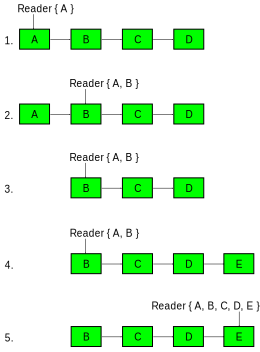
\includegraphics{defer/multver}}
\caption{Multiple RCU Data-Structure Versions}
\label{fig:defer:Multiple RCU Data-Structure Versions}
\end{figure}

하지만, 여러 버전을 유지하는 것은 더 놀라울 수도 있습니다.
예를 들어, 한 읽기 쓰레드가 동시에 업데이트 되는 링크드 리스트를 순회하는
Figure~\ref{fig:defer:Multiple RCU Data-Structure Versions} 를 고려해
봅시다.\footnote{
	RCU 링크드 리스트 API 는
	Section~\ref{sec:defer:RCU Linux-Kernel API} 에서 찾을 수 있을 겁니다.}
이 그림의 첫번째 줄에서, 읽기 쓰레드는 데이터 아이템~A 를 레퍼런스 하고 있고,
두번째 줄에서는 B 로 넘어가서, 지금까지 A 뒤에 B 가 있는 걸 봤습니다.
세번째 줄에서, 업데이트 쓰레드가 원소~A 를 지우고 네번째 줄에서 업데이트
쓰레드가 원소~E 를 리스트의 끝에 넣었습니다.
다섯번째와 마지막 줄에서, 읽기 쓰레드는 순회를 마무리 해서, 원소 A 부터 E
까지를 보게 됩니다.
\iffalse

However, maintaining multiple versions can be even more surprising.
For example, consider
Figure~\ref{fig:defer:Multiple RCU Data-Structure Versions},
in which a reader is traversing a linked list that is concurrently
updated.\footnote{
	RCU linked-list APIs may be found in
	Section~\ref{sec:defer:RCU Linux-Kernel API}.}
In the first row of the figure, the reader is referencing data item~A,
and in the second row, it advances to~B, having thus far seen A followed by~B.
In the third row, an updater removes element~A and in the fourth row
an updater adds element~E to the end of the list.
In the fifth and final row, the reader completes its traversal, having
seeing elements A through E.
\fi

그런 리스트는 존재한 적이 없었습니다.
이 상황은
Figure~\ref{fig:defer:Deletion With Concurrent Readers} 에 보인, 다른 동시의
읽기 쓰레드가 다른 버전을 보는 것보다도 더 놀라울 수 있습니다.
대조적으로,
Figure~\ref{fig:defer:Multiple RCU Data-Structure Versions} 에서는 읽기
쓰레드가 결코 존재한 적 없는 버전을 본 겁니다!
\iffalse

Except that there was no time at which such a list existed.
This situation might be even more surprising than that shown in
Figure~\ref{fig:defer:Deletion With Concurrent Readers},
in which different concurrent readers see different versions.
In contrast, in
Figure~\ref{fig:defer:Multiple RCU Data-Structure Versions}
the reader sees a version that never actually existed!
\fi

이 이상한 상황을 해결할 수 있는 한가지 방법은 완화된 semantic 을 사용하는
겁니다.
한 읽기 쓰레드의 순회는 전체 순회 동안 조재한 모든 데이터 아이템 (B, C,
그리고~D) 을 마주칠 수 있어야 하고, 이 순회의 한 순간에만 존재한 데이터 아이템
(A 와~E) 들을 만날 수도 있습니다.
따라서, 이 특수한 경우에, 읽기 쓰레드의 순회가 이 다섯 원소를 모두 만나는건
완전히 합법적입니다.
이 결과가 문제시 된다면, 이 상황을 해결하는 또다른 방법은 더 강력한 동기화
메커니즘, 예를 들면 reader-writer 락킹을 사용하는 겁니다.
물론, 더 강한 메커니즘은 더 비용이 높습니다만, 삶이란 게 선택과
트레이드오프입니다.
\iffalse

One way to resolve this strange situation is via weaker semanitics.
A reader traversal must encounter any data item that was present
during the full traversal (B, C, and~D), and might or might not
encounter data items that were present for only part of the
traversal (A and~E).
Therefore, in this particular case, it is perfectly legitimate for
the reader traveral to encounter all five elements.
If this outcome is problematic, another way to resolve this situation is
through use of stronger synchronization mechanisms, such as reader-writer
locking.
Of course, stronger mechanisms will be more expensive, but life is
about choices and tradeoffs.
\fi

이 상황이 이상하게 보이겠지만, 이는 실제 세계와 완전히 비슷합니다.
Section~\ref{sec:cpu:Overheads} 에서 봤듯이, 유한한 빛의 속도는 컴퓨터 시스템
내에서도 무시될 수 없습니다만, 시스템 바깥에서도 마찬가지입니다.
이는 결국 시스템 내에서 실제 바깥 세계에서의 것을 표현하는 모든 데이터는 낡아져
있고, 따라서 실제 세계와 일관성을 갖지 못함을 의미합니다.
결국, 실제 세계의 데이터를 다루는 알고리즘은 실제 세계의 것과 비일관적이 되는
데이터를 처리할 수 있어야만 합니다.
많은 경우에, 그런 알고리즘은 시스템 내에서의 비일관성도 완벽하게 다룰 수
있습니다.
\iffalse

Strange though this situation might seem, it is entirely consistent with
the real world.
As we saw in
Section~\ref{sec:cpu:Overheads},
the finite speed of light cannot be ignored within a computer system,
but it also cannot be ignored outside of the system.
Which in turn means that any data within the system representing
state in the real world outside of the system is outdated, and thus
inconsistent with the real world.
As a result, algorithms operating on real-world data must account for
that data being inconsistent with the real world.
In many cases, such algorithms are also perfectly capable of dealing
with inconsistencies within the system.
\fi

Section~\ref{sec:defer:Running Example} 에 있는 이 pre-BSD 패킷 라우팅 예제는
그런 관점의 예입니다.
라우팅 리스트의 컨텐츠는 라우팅 프로토콜에 의해 설정되고, 이 프로토콜은 다양한
비안정 상태를 막기 위한 상당한 지연 (초단위 또는 심지어 분단위) 을 갖습니다.
이런 지연들은 일단 라우팅 업데이트가 특정 시스템에 도달하면, 몇번은 패킷을
잘못된 방향으로 보냈을 수 있음을 의미합니다.
이 업데이트가 진행되는 수 마이크로초 동안 몇개의 패킷을 잘못된 방향으로 보내는
건 분명 문제가 아닌데, 지연된 라우팅 업데이트를 처리하는, 같거나 높은 수준의
프로토콜은 이 비일관성도 처리할 것이기 때문입니다.
\iffalse

The pre-BSD packet routing example laid out in
Section~\ref{sec:defer:Running Example}
is a case in point.
The contents of a routing list is set by routing protocols, and these
protocols feature significant delays (seconds or even minutes) to avoid
various instabilities.
These delays mean that once a routing update reaches a given system,
it might well have been sending packets the wrong way for quite some time.
Sending a few more packets the wrong way for the few microseconds during
which the update is in flight is clearly not a problem because the same
higher-level protocol actions that deal with the delayed routing updates
will also deal with the inconsistencies.
\fi

비일관성을 다루는 상황은 라우팅만이 아닙니다.
반복하지만, 시스템 외부의 상태를 추적하는 시스템 내의 데이터를 다루는 모든
알고리즘은 비일관성을 다뤄야만 하는데, 보안 정책 (많은 경우 사람이나 의원회에
의해 설정됩니다), 저장장치 설정, WiFi 액세스 포인트, 마이크로폰, 헤드셋,
카메라, 마이크, 프린터, 그외에도 많은 여러 하드웨어의 제거 등을 말해야 하는
경우들이 포함됩니다.
더 나아가서,
Figure~\ref{fig:defer:RCU Usage in the Linux Kernel} 에 보인 리눅스 커널의
레퍼런스 카운팅 사용과 결합된 리눅스 커널 RCU API 의 많은 사용예와 다른
프로젝트에서 사용이 늘어가는 해저드 포인터는 그런 비일관성에 대한 제어가
일반적으로 상상하는 것보다 훨씬 많음을 보입니다.
단일 아이템 탐색이 순회보다 더 일반적인 경우들에 특히 그렇습니다: 어쨌건,
동시의 업데이트는 전체 순회보다 단일 아이템 탐색에 영향을 덜 끼칠 겁니다.
\iffalse

Nor is Internet routing the only situation tolerating inconsistencies.
To repeat, any algorithm in which data within a system tracks
outside-of-system state must tolerate inconsistencies, which includes
security policies (often set by committees of humans), storage configuration,
and WiFi access points, to say nothing of removable hardware such as
microphones, headsets, cameras, mice, printers, and much else besides.
Furthermore, the large number of Linux-kernel RCU API uses shown in
Figure~\ref{fig:defer:RCU Usage in the Linux Kernel},
combined with the Linux kernel's heavy use of reference counting
and with increasing use of hazard pointers in other projects, demonstrates
that tolerance for such inconsistencies is more common than one might
imagine.
This is especially the case given that single-item lookups are much more
common than traversals:  After all, concurrent updates are less likely
to affect a single-item lookup than they are a full traversal.
\fi

보다 이론적인 관점에서 보자면, RCU 읽기 쓰레드들이 업데이트 쓰레드와 완전히
순서가 지어져 있다고 고려할 수 있는 특수한 경우들도 존재합니다, 이 읽기
쓰레드들은 싱글쓰레드 버전 프로그램에서와 동일한 기계 인스트럭션만을 수행함에도
불구하고 말이죠.
예를 들어,
page~\pageref{lst:defer:Insertion and Deletion With Concurrent Readers} 의
Listing~\ref{lst:defer:Insertion and Deletion With Concurrent Readers}
으로 돌아가서, 각 읽기 쓰레드가 그 삶 속에서 단 한번만 \co{access_route()} 를
수행하고 그 외에는 읽기 쓰레드와 업데이트 쓰레드 사이에 어떤 통신도 없다고
생각해 봅시다.
그러면 \co{access_route()} 의 호출 각각은 \co{access_route()} 의 line~9 에서
액세스되는 \co{route} 구조체를 생성한 \co{ins_route()} 호출 뒤로, 그리고 모든
뒤따르는 \co{ins_route()} 나 \co{del_route()} 호출 앞으로 순서지어질 겁니다.
\iffalse

From a more theoretical viewpoint, there are even some special cases where
RCU readers can be considered to be fully ordered with updaters, despite
the fact that these readers might be executing the exact same sequence of
machine instructions that would be executed by a single-threaded program.
For example, referring back to
Listing~\ref{lst:defer:Insertion and Deletion With Concurrent Readers}
on page~\pageref{lst:defer:Insertion and Deletion With Concurrent Readers},
suppose that each reader thread invokes \co{access_route()} exactly
once during its lifetime, and that there is no other communication among
reader and updater threads.
Then each invocation of \co{access_route()} can be ordered after the
\co{ins_route()} invocation that produced the \co{route} structure
accessed by line~9 of \co{access_route()} and ordered before any subsequent
\co{ins_route()} or \co{del_route()} invocation.
\fi

정리해 보면, 여러 버전을 유지하는건 RCU 읽기 쓰레드의 극단적으로 낮은
오버헤드를 가능하게 하며, 앞에서도 이야기 되었듯, 많은 알고리즘은 여러 버전들에
의해 동요하지 않습니다.
하지만, 여러 버전을 분명 다룰 수 없는 알고리즘도 존재합니다.
그런 알고리즘에 RCU 를 적용하기 위한 기술들도
있습니다만~\cite{PaulEdwardMcKenneyPhD}, 이는 이 섹션의 범위 밖입니다.
\iffalse

In summary, maintaining multiple versions is exactly what enables the
extremely low overheads of RCU readers, and as noted earlier, many
algorithms are unfazed by multiple versions.
However, there are algorithms that absolutely cannot handle multiple versions.
There are techniques for adapting such algorithms to
RCU~\cite{PaulEdwardMcKenneyPhD},
but these are beyond the scope of this section.
\fi

\paragraph{Discussion}
\label{sec:defer:Discussion}

이 예제들은 모든 업데이트 오퍼레이션이 뮤텍스를 잡고 있다고 가정을 하고 있는데,
이 말은 리스트의 버전은 한 순간에 최대 두개까지만 존재할 수 있음을 의미합니다.
\iffalse

These examples assumed that a mutex was held across the entire
update operation, which would mean that there could be at most two
versions of the list active at a given time.
\fi

\QuickQuiz{}
	리스트의 버전이 두개보다 많을 수 있도록 하기 위해서는 삭제 예제를
	어떻게 수정해야 할까요?
	\iffalse

	How would you modify the deletion example to permit more than two
	versions of the list to be active?
	\fi
\QuickQuizAnswer{
	이를 가능하게 하는 한가지 방법은
	Listing~\ref{lst:defer:Concurrent RCU Deletion} 에 보인 것처럼 하는
	것입니다.
	\iffalse

	One way of accomplishing this is as shown in
	Listing~\ref{lst:defer:Concurrent RCU Deletion}.
	\fi

\begin{listing}[htbp]
\begin{VerbatimL}
spin_lock(&mylock);
p = search(head, key);
if (p == NULL)
	spin_unlock(&mylock);
else {
	list_del_rcu(&p->list);
	spin_unlock(&mylock);
	synchronize_rcu();
	kfree(p);
}
\end{VerbatimL}
\caption{Concurrent RCU Deletion}
\label{lst:defer:Concurrent RCU Deletion}
\end{listing}

	이 코드는 여러개의 동시에 수행되는 삭제 작업들이 \co{synchronize_rcu()}
	에서 기다리게 될수도 있음을 의미합니다.
	\iffalse

	Note that this means that multiple concurrent deletions might be
	waiting in \co{synchronize_rcu()}.
	\fi
} \QuickQuizEnd

\QuickQuiz{}
	하나의 리스트는 한 순간에 RCU 버전들을 몇개까지 가질 수 있을까요?
	\iffalse

	How many RCU versions of a given list can be
	active at any given time?
	\fi
\QuickQuizAnswer{
	동기화 설계에 따라 달라집니다.
	업데이트를 보호하는 세마포어가 grace period 에 걸쳐 잡혀 있다면, 옛날
	버전과 새로운 버전, 최대 두개의 버전이 있을 수 있을 겁니다.

	하지만, 검색, 업데이트, 그리고 \co{list_replace_rcu()} 만이 락으로
	보호되고 있어서
	Listing~\ref{lst:defer:Concurrent RCU Deletion} 보인 코드에서처럼
	\co{synchronize_rcu()} 가 락의 바깥에 있다고 생각해 봅시다.
	더 나아가서 수많은 쓰레드들이 거의 동시에 RCU 교체 기능을 수행했고, 이
	읽기 쓰레드들은 또한 데이터 구조를 계속해서 지나다니고 있다고 생각해
	봅시다.
	\iffalse

	That depends on the synchronization design.
	If a semaphore protecting the update is held across the grace period,
	then there can be at most two versions, the old and the new.

	However, suppose that only the search, the update, and the
	\co{list_replace_rcu()} were protected by a lock, so that
	the \co{synchronize_rcu()} was outside of that lock, similar
	to the code shown in
	Listing~\ref{lst:defer:Concurrent RCU Deletion}.
	Suppose further that a large number of threads undertook an
	RCU replacement at about the same time, and that readers
	are also constantly traversing the data structure.
	\fi

	그러면 다음과 같은 일련의 이벤트들이
	Figure~\ref{fig:defer:RCU Replacement in Linked List} 의 마지막
	상태로부터 발생할 수 있습니다.
	\iffalse

	Then the following sequence of events could occur, starting from
	the end state of
	Figure~\ref{fig:defer:RCU Replacement in Linked List}:
	\fi

	\begin{enumerate}
	\item	쓰레드~A 가 리스트를 횡단하면서 5,2,3 원소로의 레퍼런스를
		얻습니다.
	\item	쓰레드~B 가 5,2,3 원소를 새로운 5,2,4 원소로 교체하고, 자신의
		\co{synchronize_rcu()} 호출이 리턴하길 기다립니다.
	\item	쓰레드~C 가 리스트를 횡단하면서 5,2,4 원소로의 레퍼런스를
		얻습니다.
	\item	쓰레드~D 가 5,2,4 원소를 새로운 5,2,5 원소로 교체하고, 자신의
		\co{synchronize_rcu()} 호출이 리턴하길 기다립니다.
	\item	쓰레드~E 가 리스트를 횡단하면서 5,2,5 원소로의 레퍼런스를
		얻습니다.
	\item	쓰레드~F 가 5,2,5 원소를 새로운 5,2,6 원소로 교체하고, 자신의
		\co{synchronize_rcu()} 호출이 리턴하길 기다립니다.
	\item	쓰레드~G 가 리스트를 횡단하면서 5,2,6 원소로의 레퍼런스를
		얻습니다.
	\item	그리고 앞의 두 스텝들이 빠르게 계속해서 반복되어서 모든
		쓰레드들이 \co{synchronize_rcu()} 호출이 리턴하길 기다립니다.
	\end{enumerate}
	\iffalse

	\item	Thread~A traverses the list, obtaining a reference to
		the 5,2,3 element.
	\item	Thread~B replaces the 5,2,3 element with a new
		5,2,4 element, then waits for its \co{synchronize_rcu()}
		call to return.
	\item	Thread~C traverses the list, obtaining a reference to
		the 5,2,4 element.
	\item	Thread~D replaces the 5,2,4 element with a new
		5,2,5 element, then waits for its \co{synchronize_rcu()}
		call to return.
	\item	Thread~E traverses the list, obtaining a reference to
		the 5,2,5 element.
	\item	Thread~F replaces the 5,2,5 element with a new
		5,2,6 element, then waits for its \co{synchronize_rcu()}
		call to return.
	\item	Thread~G traverses the list, obtaining a reference to
		the 5,2,6 element.
	\item	And the previous two steps repeat quickly, so that all
		of them happen before any of the \co{synchronize_rcu()}
		calls return.
	\end{enumerate}
	\fi

	따라서, 얼마든지 많은 버전들이 존재할 수 있습니다만, 메모리 크기와
	얼마나 많은 업데이트들이 하나의 grace period 안에 완료될 수 있느냐에 그
	수가 제한됩니다.
	하지만 그렇게 자주 업데이트 되는 데이터 구조체들은 RCU 를 사용하기에
	적합한 후보가 아닐 수 있음을 알아두시기 바랍니다.
	그렇다곤 해도, RCU 는 필요할 때에는 높은 비율의 업데이트를 처리할 수
	있습니다.
	\iffalse

	Thus, there can be an arbitrary number of versions active,
	limited only by memory and by how many updates could be completed
	within a grace period.
	But please note that data structures that are updated so frequently
	probably are not good candidates for RCU.
	That said, RCU can handle high update rates when necessary.
	\fi
} \QuickQuizEnd

\subsubsection{Summary of RCU Fundamentals}
\label{sec:defer:Summary of RCU Fundamentals}

이 섹션에서는 RCU 기반 알고리즘의 세가지 기본 컴포넌트를 설명했습니다:
\iffalse

This section has described the three fundamental components of RCU-based
algorithms:
\fi

\begin{enumerate}
\item	새로운 데이터의 추가를 위한 공개-구독 메커니즘,

\item	전부터 존재했던 RCU 읽기 쓰레드들이 종료되기를 기다리는 방법 (자세한
	내용은 Section~\ref{sec:memorder:RCU} 을 참고하세요), 그리고

\item	동시에 수행중인 RCU 읽기 쓰레드들에 피해를 주거나 너무 오래 기다리게
	하지 않고 변화를 가할 수 있도록 여러 버전을 관리하는 방법.
\iffalse

\item	a publish-subscribe mechanism for adding new data,

\item	a way of waiting for pre-existing RCU readers to finish
	(see Section~\ref{sec:memorder:RCU} for more detail),
	and

\item	a discipline of maintaining multiple versions to permit
	change without harming or unduly delaying concurrent RCU readers.
\fi
\end{enumerate}

\QuickQuiz{}
	\co{rcu_read_lock()} 과 \co{rcu_read_unlock()} 함수는 스핀하지도
	블락하지도 않는데 어떻게 RCU 업데이트 쓰레드들이 RCU 읽기 쓰레드들을
	대기시킬 수가 있나요?
	\iffalse

	How can RCU updaters possibly delay RCU readers, given that the
	\co{rcu_read_lock()} and \co{rcu_read_unlock()}
	primitives neither spin nor block?
	\fi
\QuickQuizAnswer{
	특정 RCU 업데이트 쓰레드에 의해 가해진 수정사항은 연관된 CPU 가 해당
	데이터를 포함하는 캐시 라인들을 무효화 하도록 만들 것이고, 동시에
	수행중인 RCU 읽기 쓰레드들을 수행중인 해당 CPU 들이 비싼 캐시 미스를
	마주하게 만들 겁니다.
	(동시에 수행중인 읽기 쓰레드에게 비싼 캐시 미스를 만들지 않고 데이터
	구조에 변경을 가할 수 있는 알고리즘을 설계할 수 있을까요?
	또는 뒤따르는 읽기 쓰레드들에게?)
	\iffalse

	The modifications undertaken by a given RCU updater will cause the
	corresponding CPU to invalidate cache lines containing the data,
	forcing the CPUs running concurrent RCU readers to incur expensive
	cache misses.
	(Can you design an algorithm that changes a data structure
	\emph{without}
	inflicting expensive cache misses on concurrent readers?
	On subsequent readers?)
	\fi
} \QuickQuizEnd

이 세개의 RCU 컴포넌트는 동시에 수행되는 읽기 쓰레드에 상관 없이 데이터가
업데이트 되도록 하고, 놀랍도록 다양한, 다른 종류의 RCU 기반의 알고리즘들을
구현하는 다른 방법들로 조합될 수 있습니다.
따라서, 다음 섹션에서는 리눅스 커널 API 를 설명할텐데, 리스트와 같은 간단한
데이터 구조가 포함됩니다.
\iffalse

These three RCU components
allow data to be updated in face of concurrent readers, and
can be combined in different ways to
implement a surprising variety of different types of RCU-based algorithms.
However, it is usually better to work at higher levels of abstraction.
To this end, the next section describes the Linux-kernel API, which
includes simple data structures such as lists.
\fi
